\section{Gewöhnliche DGL}

\vspace{1\baselineskip}

\Definition{

    Eine gewöhnliche DGL heisst \fat{autonom}, wenn $f$ unabhängig von $t$ ist.
}

\vspace{1\baselineskip}

\fat{Umwandlung in DGL erster Ordnung}

Gegeben: $\vec{y}_n = \vec{f} \klammer{t,\vec{y},\dots,\vec{y}^{(n-1)}}$

Vorgehen:
\begin{enumerate}
    \item Schreibe einen Vektor mit Einträgen $\vec{y}(t),\dots,\vec{y}^{(n-1)}(t)$:
            $$
                \vec{z}(t) = \begin{pmatrix}
                    \vec{z_0} \\ \vdots \\ \vec{z}_{n-1} (t)
                \end{pmatrix}
                := \begin{pmatrix}
                    \vec{y} (t) \\ \vdots \\ \vec{y}^{(n-1)}
                \end{pmatrix}
            $$
    \item Leite diesen Vektor ab und setze die DGL ein:
            $$
                \frac{d}{dz} \vec{z} (t) = \begin{pmatrix}
                    \vec{y}' \\ \vdots \\ \vec{y}^{(n)} (t)
                \end{pmatrix} = \begin{pmatrix}
                    \vec{z}_1 (t) \\ \vdots \\ \vec{y}^{(n-1)} (t) \\ \vec{f}(t,\vec{y},\dots,\vec{y}^{(n-1)})
                \end{pmatrix}
                =: \vec{g}(t,\vec{z})
            $$
\end{enumerate}

\vspace{1\baselineskip}

\fat{Autonomisierung einer DGL}

Hat man eine DGL erster Ordnung $\dot{\vec{y}} = \vec{f}(t,\vec{y})$ mit $\vec{y} \in \R^n$,
so kann man di Zeitabhängigkeit in die DGL einpacken. Das Vorgehen ist genau analog zur
Umwandlung in eine DGL erster Ordnung. Dazu wird $\vec{z} \in \R^{n+1}$ eingeführt:
$$
    \vec{z} (t) := \begin{pmatrix}
        \vec{y} (t) \\ t
    \end{pmatrix}
    =
    \begin{pmatrix}
        \vec{z} \\ z_{n+1}
    \end{pmatrix}
$$
Somit erhalten wir die autonome DGL:
$$
    \dot{\vec{z}} (t) = \begin{pmatrix}
        \vec{f} (z_{n+1} , \vec{z}) \\ 1
    \end{pmatrix}
    =: \vec{g} (\vec{z})
$$

\vspace{1\baselineskip}

\fat{Konvergenzordnung}

Sei $p > 0$ die Konvergenzordnung des Verfahrens sodass $\forall N \in \N \ : \
E(N) \leq \frac{c}{N^p}$ bzw $E(h) \leq c h^p$ mit $h:= \frac{t_{\text{end}} - t_{0}}{N}$
und einer Konstanten $c$. Berechnung: $E(N) \approx c N^{-p} \Leftrightarrow
\log(E(N)) \approx \log(c) - p \log(N)$ $\Leftrightarrow$ Plot von $E$ gegen $N$ in einem
LogLog-Plot ist eine Gerade mit Steigung $-p$

\vspace{1\baselineskip}

\fat{Vorgehen} (Bestimmung der Konvergenzordnung)

- Verwende das Verfahren und löse die DGL mehrmals für verschiedene $N$.

- Berechne für jedes $N$: $e(N) := \Norm{\vec{y}_{\text{exact}} - \vec{y}_N}$

- Berechne:

$p = - \text{polyfit} (\log(N) , \log(e), 1)[0] = \text{polyfit} (\log(h),\log(e),1)[0]$

\vspace{1\baselineskip}

\underline{\fat{Polygonzugverfahren}}

Gegeben: $\dot{\vec{y}} = \vec{f}(t,\vec{y})$, $\vec{y}(t_0) = \vec{y}_0$

Gesucht: Lösung $y(t)$ des AWP 1. Ordnung

\vspace{1\baselineskip}

\fat{Explizites Eulerverfahren}

Approximation durch Tangende zum Anfangszeitpunkt $t_k$.

$\vec{y}_{k+1} := \vec{y}_k + h_k \vec{f}(t_k,\vec{y}_k)$

Lokaler Fehler: $O(h^2)$

\begin{center}
    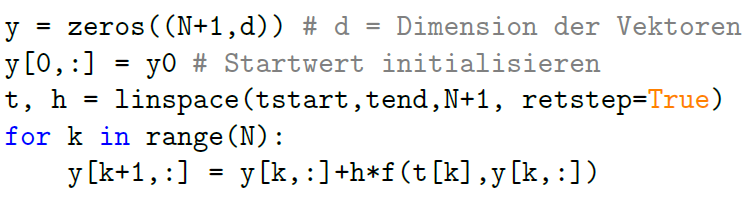
\includegraphics[width=0.3\textwidth]{Figures/eE.png}
\end{center}

\vspace{1\baselineskip}

\fat{Implizites Eulerverfahren}

Approximation durch Tangente am nächsten Zeitpunkt $t_{k+1}$.

$\vec{y}_{k+1} := \vec{y}_k + h_k \vec{f}(t_{k+1} , \vec{y}_{k+1})$

$\Rightarrow \vec{y}_{k+1}$ NST von: $F(\vec{X}) := \vec{X} - \vec{y}_k - h_k \vec{f}(t_{k+1},\vec{X})$


Guter Startwert für Nullstellensuche: Schritt aus eE

Implizit bedeutet, dass für $\vec{y}_{k+1}$ eine (i.A. nichtlineare) Gleichung aufgelöst
werden muss.

Lokaler Fehler: $O(h^2)$

\begin{center}
    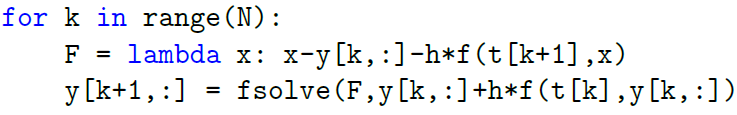
\includegraphics[width=0.31\textwidth]{Figures/iE.png}
\end{center}

\vspace{1\baselineskip}

\fat{Implizite Mittelpunktregel}

Approximation durch Tangente zum Zeitpunkt $(t_k + t_{k+1})/2$

$\vec{y}_{k+1} := \vec{y}_k + h_k \vec{f}(\frac{1}{2}(t_k+t_{k+1}),\frac{1}{2}(\vec{y}_k + \vec{y}_{k+1}))$

$\Rightarrow \vec{y}_{k+1}$ NST von: $F(\vec{X}) := \vec{X} - \vec{y}_k - h_k \vec{f}(\frac{1}{2}(t_k + t_{k+1}),\frac{1}{2}(\vec{y}_k + \vec{X}))$

Guter Startwert für Nullstellensuche: Schritt aus eE

\vspace{1\baselineskip}

Lokaler Fehler: $O(h^3)$

\begin{center}
    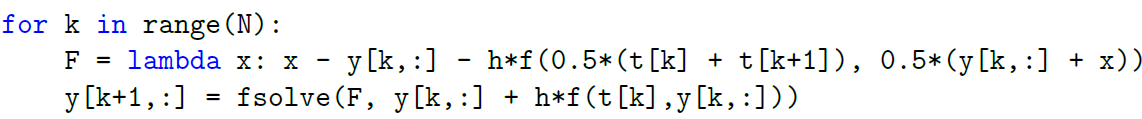
\includegraphics[width=0.48\textwidth]{Figures/iM.png}
\end{center}

\vspace{1\baselineskip}

\fat{Implizite Trapezregel}

$\vec{y}_{k+1} = \vec{y}_k + \frac{h}{2} \klammer{\vec{f}(t_k,\vec{y}_k) + \vec{f}(t_{k+1} , \vec{y}_{k+1})}$

$\Rightarrow y_{k+1}$ NST von: $F(\vec{X}) = \vec{X} - \vec{y}_k - \frac{h}{2} \klammer{\vec{f}(t_k,\vec{y}_k) + \vec{f}(t_{k+1} , \vec{X})}$

Guter Startwert für Nullstellensuche: Schritt aus eine

Lokaler Fehler: $O(h^3)$

\vspace{1\baselineskip}

\underline{\fat{Störmer-Verlet-Verfahren}}

Geg.: $\ddot{\vec{y}} = \vec{f}(t,\vec{y})$ (keine $\dot{\vec{y}}$ Abhängigkeit!),
$\vec{y} (t_0) = \vec{y}_0$, $\dot{\vec{y}}(t_0) = \vec{v}_0$

Ges. Lösung $\vec{y}(t)$ des AWP 2. Ordnung

\vspace{1\baselineskip}

\fat{Zwei-Schritt-Verfahren}

Idee: Approximation durch eine Parabel und äquidistante $t_k$

Idee: $f(t_k , y_k) = \ddot{y}_k \approx \frac{\dot{y}_{k+1} - \dot{y}_k}{h} \approx
\frac{\frac{y_{k+1} - y_k}{h} - \frac{y_k - y_{k-1}}{h}}{h} \approx
\frac{y_{k+1} - 2 y_k + y_{k-1}}{h^2}$

$\vec{y}_{k+1} := - y_{k-1} + 2 \vec{y}_k + h^2 \vec{f}(t_k , \vec{y}_k)$

mit zweitem Startwert: $\vec{y}_1 = \vec{y}_0 + h \vec{v}_0 + \frac{h^2}{2} \vec{f}(t_0,\vec{y}_0)$

\begin{center}
    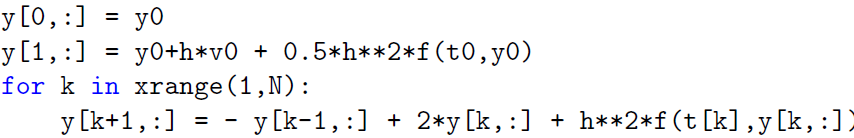
\includegraphics[width=0.35\textwidth]{Figures/ZSF.png}
\end{center}

\vspace{1\baselineskip}

\fat{Ein-Schritt-Verfahren}

Idee: $\ddot{\vec{y}} = \vec{f}(t,\vec{y}) \Leftrightarrow \dot{\vec{y}} = \vec{v}$ und
$\dot{\vec{v}} = \vec{f}(t,\vec{y})$

Verwende das eE für $\dot{\vec{y}}(t) = \vec{v}(t)$ und
$\dot{\vec{v}}(t) = \vec{f}(t,\vec{y})$

Es gibt 2 Methoden: Leap-Frog-Methode und Velocity-Verlet

\vspace{1\baselineskip}

\fat{Leap-Frog-Methode}

$\vec{v}_{k+\frac{1}{2}} := \vec{v}_{k-\frac{1}{2}} + h \vec{f}(t_k,\vec{y}_k)$

$\vec{y}_{k+1} := \vec{y}_k + h \vec{v}_{k+\frac{1}{2}}$

mit Startwert $\vec{v}_{\frac{1}{2}} = \vec{v}_0 + \frac{h}{2} \vec{f}(t_0,\vec{y_0})$

\begin{center}
    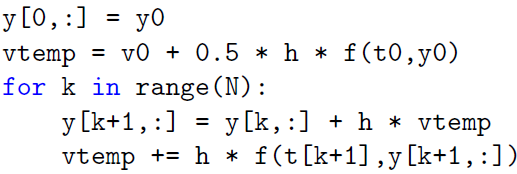
\includegraphics[width=0.2\textwidth]{Figures/ESF.png}
\end{center}

\vspace{1\baselineskip}

\fat{Velocity-Verlet}

$\vec{y}_{k+1} := \vec{y}_k + h \vec{v}_k + \frac{h^2}{2} \vec{f}(t_k,\vec{y}_k)$

$\vec{v}_{k+1} := \vec{v}_k + \frac{h}{2} \klammer{\vec{f}(t_k,\vec{y}_k) + \vec{f}(t_{k+1},\vec{y}_{k+1})}$

\begin{center}
    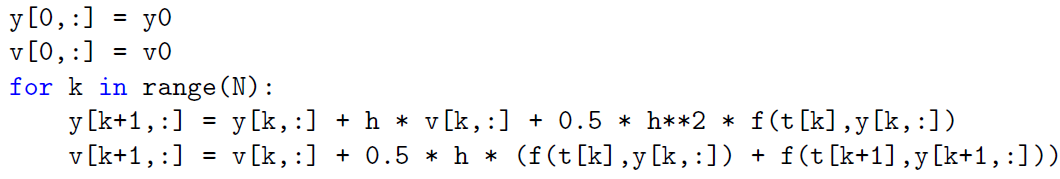
\includegraphics[width=0.4\textwidth]{Figures/VV.png}
\end{center}

Im Gegensatz zu Leap-Frog liefert Vel.Verl. die Geschw. bei $t_k$.

\vspace{1\baselineskip}

Die Einschritt-Verfahren sind numerisch stabiler.

In allen Störmer-Verlet-Verfahren ist die Energie erhalten.

Code im Skript auf Seite 80

\vspace{1\baselineskip}

\fat{Konvergenzordnung}

Wie bei Quadratur.

Exacte Lösung: ode45

from ODE45 import ODE45

$t,y =$ ode45$(f,(t_0,t_{\text{end}}),y_0)$

\vspace{1\baselineskip}

\underline{\fat{Fehler}}
\begin{itemize}
    \item Lokaler Fehler: $\Norm{y(t_{n+1}) - y_{n+1}}$ abschätzen durch fixe Konstanten.
    \item Fehlerfortpflanzung: $\Norm{y_{n+1}^{\star} - y_{n+1}}$ abschätzen mit $y(t_n)$
            und $y_n$.
            Methode: Approximiere $y_{n+1}^{\star}$ mit $y_n$ und $y_{n+1}$ mit $y(t_n)$
    \item Fehlerakkumulierung: Über die Fehlerfortpflanzung bis $n$ summieren. Die Potenz
            nicht vergessen. Tipp: Geometrische Reihe.
\end{itemize}

\vspace{1\baselineskip}

\Theorem{

    $\Norm{\vec{y}_n - \vec{y}(t_n)} \leq M \cdot h$ für alle $n$, wobei

    $M = \frac{1}{L} \klammer{e^{L(T-t_0)} -1} \frac{1}{2} \max \Norm{\ddot{\vec{y}}(t)}$
    \ \ für $t \in [t_0,T]$.

    Kann man mittels den vorherigen drei Fehlertypen beweisen.
}
